\section{Streaming}
\subsection{Gstreamer}
\label{sec:gstreamer}
As described in Section~\ref{sec:tools_streaming} the tool GStreamer is used for reading the drones' video feed and forwarding it to CRTMP.
Gstreamer is a pipeline based tool, and has a command line version which can be executed using \verb+gst-launch-0.10+.
The plugins the pipeline consist of are seperated by a \verb+!+.
The first plugin in the pipeline is called a source element, and the final element a sink.
The plugins between the source and sink element consist of a set of video and audio processing-, and data management plugins.
A sample pipeline is illustrated in Figure~\ref{fig:sample_pipeline}.

\begin{figure}[htb]
    \centering
    
\includegraphics[width=\textwidth]{gfx/sample_pipeline.pdf}
    \caption{Illustration of a sample pipeline.}
    \label{fig:sample_pipeline}
\end{figure}

The source element is capable of receiving a video feed over a specific protocol from a defined destination.
As described in Appendix~\ref{app:ar_drone_specification} the drone outputs its video feed using the TCP protocol on port 5555, and its IP-address is 192.168.1.1.
To read the stream, the GStreamer plugin \verb+tcpclientsrc+ is used.
The parameters \verb+host+ and \verb+port+ can be set for \verb+tcpclientsrc+. 
The first part of the pipeline can be seen in Listing~\ref{lst:tcpclientsrc}.

\begin{lstlisting}[style=sourceCode, language=C, caption=Partial Gstreamer pipeline illustrating tcpclientsrc, label=lst:tcpclientsrc]
gst-launch-0.10 tcpclientsrc host=192.168.1.1 port=5555
\end{lstlisting}

The data available to the next plugin are H.264 encoded video with PaVE headers.
The PaVE headers are parsed using the paveparse plugin \citep{paveparse}, as described in Section~\ref{sec:tools_streaming}.
Paveparse removes the PaVE headers and send the remaining H.264 data down the pipeline.
Furthermore is ignores lost frames and discards frames sent out of order to reduce delay on the stream.
This is necesarry as the drone streams over TCP, and as described in Section \fxfatal{Ref til analysis om hvorfor no delay p� streamen er vigtigt, og check at s�tningen stadig giver mening} delay is not acceptable on the stream. \\

As specified in Section~\ref{sec:technologies} the video output of GStreamer should be in FLV so that the Flash application in \deno{B} can display it.
Two pipelines that output FLV can be created.
The first is using a H.264 decoder to create raw video data, and then encode it as FLV.
The second is using FLVmux.
FLVmux muxes audio and video streams into a single flv file \citep{flvmux}.
However, as the H.264 data has no headers, due to \textit{paveparse}, the H.264 decoder cannot decode the video.
Therefore an FLVmuxer is used to create FLV output. \\

With FLV video outputted from the FLVmuxer, the sink-element can be added to the pipeline.
As the video feed is forwarded to CRTMP, the sink element is \verb+rtmpsink+.
It has one parameter called \verb+location+, which is the URL-address of the RTMP server with an extension specifying the source-URL of the stream on the RTMP server.
The \verb+rtmpsink+ can be seen in Listing~\ref{lst:rtmpsink}:

\begin{lstlisting}[style=sourceCode, language=C, caption=Partial Gstreamer pipeline illustrating rtmpsink, label=lst:rtmpsink]
rtmpsink location='rtmp://0.0.0.0/live/myStream'
\end{lstlisting}

The pipeline that forwards the video feed from the drones can be seen in Listing~\ref{lst:pipeline1}.

\begin{lstlisting}[style=sourceCode, language=C, caption=Gstreamer Pipeline with tcpclientsrc and rtmpsink, label=lst:pipeline1]
tcpclientsrc host=192.168.1.1 port=5555 ! paveparse ! flvmux ! rtmpsink location='rtmp://0.0.0.0/live/myStream'
\end{lstlisting}

To handle plugins working at different speeds data management plugins are added to the pipeline.
The plugin used is \verb+queue+.
\verb+queue+ is a data queue that queues data until e.g. the queue reaches a specified size \citep{gstreamer_plugins_queue}.
The \verb+queue+ element is added between every plugin except \verb+tcpclientsrc+ and \verb+paveparse+.  \\

The complete pipeline can be seen in Listing~\ref{lst:pipeline2}: 

\begin{lstlisting}[style=sourceCode, language=C, caption=Complete Gstreamer Pipeline, label=lst:pipeline2]
tcpclientsrc host=192.168.1.1 port=5555 ! paveparse ! queue ! flvmux ! queue ! rtmpsink location='rtmp://0.0.0.0/live/myStream'
\end{lstlisting}

\subsection{C++ RTMP Server}
\label{sec:CRTMP}
As described in \ref{sec:tools_streaming} C++ RTMP Server is used as the server tool between GStreamer and the Flash application in the \deno{B}. \\

%CRTMP is found at http://www.rtmpd.com and comes in a source package ready to run.
%CRTMP is a standard executable binary. \\

There are four ways to run CRTMP:

\begin{itemize}
   \item run\_all.sh
   \item run\_all\_deamon.sh
   \item run\_flvplayback.sh
   \item run\_flvplayback\_deamon.sh
\end{itemize}

If \verb+sh run_all.sh+ is run, CRTMP will start using the configuration file \verb+all.lua+.
The flvplayback was used, because this is the flash streamer application.
The configuration file \verb+flvplayback.lua+ was configured as seen in listing~\ref{lst:flvplayback}.

\begin{lstlisting}[style=sourceCode, language=C, caption=flvplayback.lua configuration, label=lst:flvplayback]
acceptors =
  {
    {
      ip="0.0.0.0",
      port=1935,
      protocol="inboundRtmp"
    }
  },
externalStreams =
  {
    {
      uri="rtmp://flash.oit.duke.edu/vod/MP4:test/brunswick.m4v",
      localStreamName="test",
      forceTcp=true
    }
  },
\end{lstlisting}


\verb+Acceptors+ define inbound- and \verb+externalStreams+ outbound connections of CRTMP.
Inbound defines which ports CRTMP will let users connect to and \verb+externalStreams+ is the source of the stream.
The sample \verb+externalSteam+ seen in listing~\ref{listing:flvplayback} has a video file on an external server as input, and gives the outbound stream the name \verb+test+.
This test-source was used to test if CRTMP was running correctly.
To view the stream, the program Video Lan Client \emph{[VLC]}, was used, as it has the same capabilities as flash in regard to streaming RTMP.

A connection is established with a URL-address of the format seen in Listing~\ref{lst:server_address}, where the \verb+server address+ is the address of the CRTMP server, the \verb+application+ is the application where CRTMP lookup e.g. live or media, and the \verb+streamName+ is the name of the stream.

\begin{lstlisting}[style=sourceCode, language=C, caption=CRTMP URL Format, label=lst:server_address]
rtmp://[server address]/[application]/[streamName]
\end{lstlisting}

When a user connects to CRTMP and the \verb+application+ is live, CRTMP will try to find a live stream that correspond to the link name.
If no such live streams is found, CRTMP will look in the media folder and try to find file streams.
If no file stream is found, CRTMP will wait for the live stream \verb+streamName+. \\

C++ RTMP Server also uses RSA keys.
It is possible to make users and add these users to realms. 
This can be used as an extra layer of security, but it is not implemented in this version of \projectname{}.

\section{Output stream}
Following the setup of GStreamer and CRTMP, the next step is reading the output stream and displaying it in a Flash application.
Due to the PaVE headers, however, this is not possible.

\subsection{Issues with PaVE Headers}
\label{sec:issues_with_pave_headers}
The documentation for the PaVE headers can be found at \citep[page. 59-60]{ardrone_developer_guide}.
As described in Section~\ref{sec:gstreamer}, Flash applications are unable to interpret the PaVE headers. 
As a result of this, they are unable to display a video stream encoded with them.
These headers must therefore be removed or replaced with another header to make the stream readable.
The implemented solution removes them with the \verb+paveparse+ plugin, described in Section~\ref{sec:gstreamer}.
Removing the header leaves raw video data with no information about how to interpret it.
As a result of this, the Flash application, VLC, or any other video players is unable to interpret the raw video data.
An illustration of the PaVE header problem can be seen in Figure~\ref{fig:videoframe}. \\

\begin{figure}[htb]
    \centering
    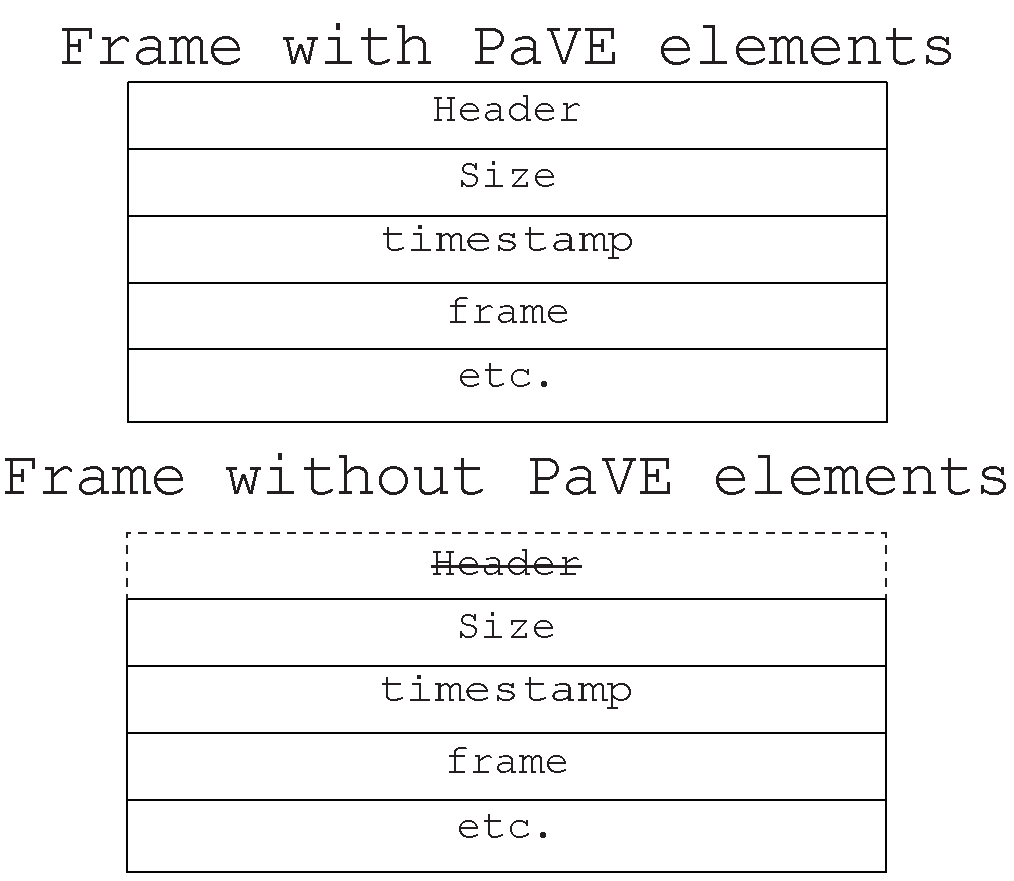
\includegraphics[width=0.7\textwidth]{gfx/videoframe.pdf}
    \caption{Illustration of videoframes with and without PaVe headers.}
    \label{fig:videoframe}
\end{figure}

The PaVE headers result in a situation that makes displaying the video stream in Flash impossible, as the video feed cannot be interpreted by a Flash application neither with nor without them.

\subsection{Test input}
The designed solution would work if the drones' video feed used a standard header format in the raw video feed.
This can be documented by using a different video source.
For this purpose the GStreamer plugin \verb+videotestsrc+ is used.
It creates a test video stream as seen in figure~\ref{fig:videotestsrc}, consisting of raw video data. \\

If this test-source is used instead of the one that is streamed from the drone, it is possible to show that this solution will work.
The issue is the video format of the video stream from the drone. \\

This solution can be seen in figure~\ref{fig:working_solution}. \\

\begin{figure}[htb]
    \centering
    
\includegraphics[width=0.6\textwidth]{gfx/testvideosrc.pdf}
    \caption{The test video source played with a Flash application.}
    \label{fig:testvideosrc}
\end{figure}

\begin{figure}[htb]
    \centering
    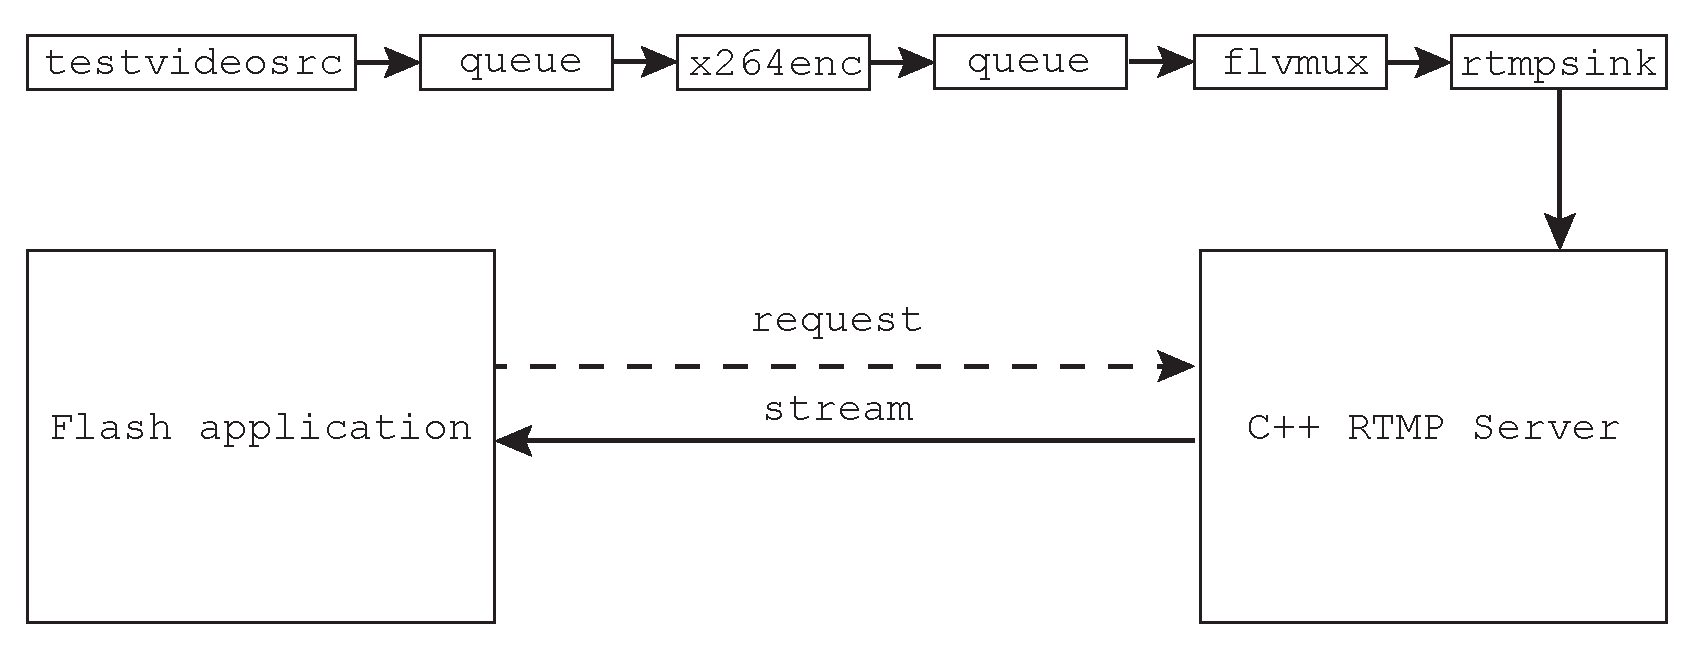
\includegraphics[width=\textwidth]{gfx/Working_solution.pdf}
    \caption{Illustration of the working solution with use of the video test source.}
    \label{fig:working_solution}
\end{figure}

\subsection{Implemented solution}
\label{sec:video_stream_implemented_solution}
The streaming setup used in \projectname{} uses only GStreamer.
One pipeline that reads the drones' video feed and serves as a server, denoted \deno{SP}, and a client pipeline, denoted \deno{CP}, for displaying the video feed on the client side.
The setup can be seen in Figure~\ref{fig:current_solution}.

\begin{figure}[htb]
    \centering
    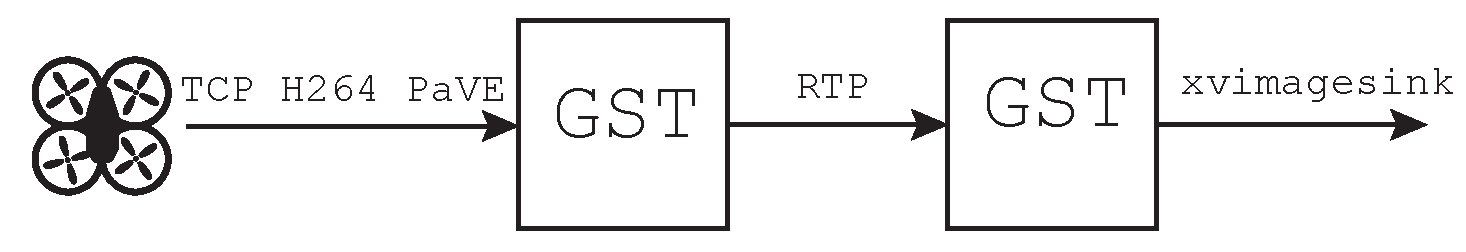
\includegraphics[width=\textwidth]{gfx/current_solution.pdf}
    \caption{Illustration of the current solution with xvimagesink.}
    \label{fig:current_solution}
\end{figure}

\deno{SP} reads the drones' video feed and multicasts it using the Real-time Transport Protocol (RTP).
RTP is a standardized protocol for sending audio and video packages over an IP network.
RTMP is not used, as it is a protocol made specifically for Flash.
For a GStreamer only solution, RTP is better choice as it is simpler to set up, since it does not have to include settings for the Flash application.
RTP packages are sent via UDP.
\deno{SP} uses the \verb+tcpclientsrc+ and \verb+paveparse+ plugins used described in Section~\ref{sec:gstreamer}. \\

Video data send via RTP must be pay-loaded, as a video frame is larger than the maximum size allowed size of a UDP packet.
Pay-loading a video stream means encapsulating it into a specific format.
Pay-loading adds the RTP header to the data packages which encapsulates the pay-loaded data.
GStreamer has a set of RTP pay- and depayloaders for each video format it supports.
The plugin used in this pipeline is \verb+rtph264pay+. \\

GStreamer does not have a dedicated RTP sink.
As RTP packages are sent via UDP, the \verb+udpsink+ is used.
\verb+udpsink+ has two parameters, \verb+host+ and \verb+port+, and a set of optional flags with default values.
The flag \verb+auto-multicast+ must be set to true to broadcast the stream globally.
Accordingly the host is set to the multicast IP \verb+224.1.1.1+.
The port is set to \verb+5123+. \\ %as specified in Section\fxfatal{ref til der hvor det kommer}.

The complete \deno{SP} can be seen in Listing~\ref{lst:SP}:

\begin{lstlisting}[style=sourceCode, language=C, caption=rtmpsink setup, label=lst:SP]
tcpclientsrc host=192.168.1.1 port=5555 ! paveparse ! rtph264pay ! udpsink host=224.1.1.1 port=5123 auto-multicast=true
\end{lstlisting}

\deno{CP} uses the \verb+udpsrc+ element to read the video stream.
\verb+udpsrc+ parameters are identical to those of \verb+udpsink+.
In order to decode the stream, an additional parameter named \verb+caps+ must be set.
\verb+caps+ are used to describe metadata about the incoming video stream and contains information such as encoding, the protocol it is being sent using, framerate, etc.
The caps are generated by \deno{SP}.
The \verb+udpsrc+ element of \deno{CP} can be seen in Listing~\ref{lst:udpsrc}. \\

\begin{lstlisting}[style=sourceCode, language=C, caption=udpsrc Setup, label=lst:udpsrc]
udpsrc uri=rtp://XXX.XXX.XXX.XXX port=5123 caps = "application/x-rtp, media=(string)video, clock-rate=(int)90000, encoding-name=(string)H264, sprop-parameter-sets=(string)\"Z01AFeygoP2AiAAAAwALuaygAHixbLA\\=\\,aOvssg\\=\\=\", payload=(int)96, ssrc=(uint)1171155755, clock-base=(uint)868988588, seqnum-base=(uint)65233"
\end{lstlisting}
%\fxfatal{Highlighting er m�rkelig i streaming listings}.

The next two steps of the pipeline is depayload the received data and decode it to raw video data.
The depayloading is done with the \verb+rtph264depay+ plugin and the decoding with the \verb+ffdec_h264+ plugin.
Following these two steps, the video data is reassembled after the transfer and been decoded.
The last plugin used is \verb+xvimagesink+ which displays the video stream to the user.
\verb+xvimagesink+ has two flags used to remove delay on the stream named \verb+sync+ and \verb+async+ which are both set to true.
The complete \deno{CP} can be seen in Listing~\ref{lst:CP}. \\

\begin{lstlisting}[style=sourceCode, language=C, caption=Client Pipeline, label=lst:CP]
udpsrc uri=rtp://XXX.XXX.XXX.XXX port=5123 caps = "application/x-rtp, media=(string)video, clock-rate=(int)90000, encoding-name=(string)H264, sprop-parameter-sets=(string)\"Z01AFeygoP2AiAAAAwALuaygAHixbLA\\=\\,aOvssg\\=\\=\", payload=(int)96, ssrc=(uint)1171155755, clock-base=(uint)868988588, seqnum-base=(uint)65233" ! rtph264depay ! ffdec_h264 ! xvimagesink sync=false async=false
\end{lstlisting}

This solution allows us to display the video stream in a separate player, such as VLC, on the clients computer. 



%% http://wiki.rtmpd.com/documentation (Maybe this should in bib)